\documentclass[10pt]{article}\usepackage[margin=.65in]{geometry}\usepackage[T1]{fontenc}\usepackage{graphicx}\setlength{\parindent}{0pt}\setlength{\parskip}{7pt}\sloppy\begin{document}{\large Literal word batch inversion under fast-branch guards}\par Three main declarations compile. FastBatch.product is the literal (norm*s1)\%p UInt64 operation; both is the existing proved widened-modpow inverse generator at p-2; ni and si multiply both by s1 and norm respectively with the same UInt64 reduction order as native lines1028–1030. guarded\_product derives canonical, nonzero product from canonical nonzero operands, primality and the explicit p$<$2\textasciicircum{}31 bound. Thus the native inverse assertion has its required nonzero input. batch\_decode proves all three returned words canonical and decodes both=(N*S1)\textasciicircum{}-1, ni=N\textasciicircum{}-1, si=S1\textasciicircum{}-1.\par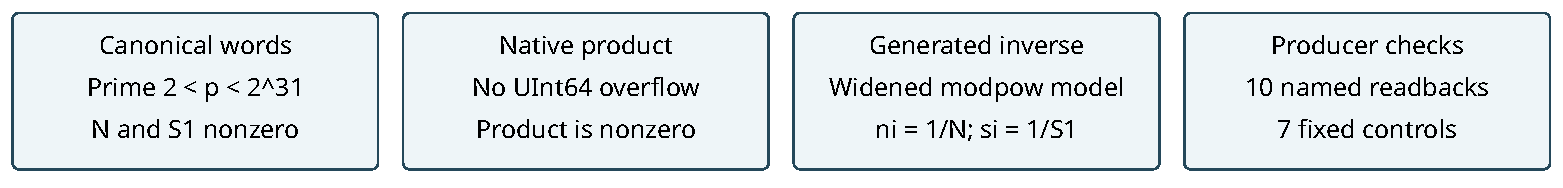
\includegraphics[width=\linewidth]{diagram.pdf}\par Native source inspected: three\_leads.rs194–205 bm/bi;210–226 mul dispatch;306 onward inv dispatch;588–599 modpow with widened u128 multiplication;1024–1030 batch guard/body. Source SHA256 26e99b56dace8f848d055e8709bb989622e4caea65aec26d63e00805153dc3c6. For correspondence, Field.n=1 and diagnostic tables absent are explicit source-dispatch restrictions. The proof requires prime p and 2$<$p$<$2\textasciicircum{}31, excluding the earlier binary branch. Canonical input bounds and actual nonzero word guards are assumptions, not outputs of a modeled norm/s1 prelude. Physical counter/allocator/compiler semantics remain separate.

The proof reuses pinned Inversion.lean generator\_product/generator\_decode, Wide.lean widened multiplication and exponent loop, WordErrorExclusion canonical-word-nonzero, and uint64\_mul\_decode/canonical. There is no inverse witness supplied by the caller: the modeled generator computes the inverse. The final field simplification is a separate field\_batch identity. Arbitrary malformed inputs are not modeled as successful native execution merely because the total Lean arithmetic body has a value.

Checks: FastBatchInverse-attempt-HIoyqSdY, FastBatchControls-attempt-eCuMmjrA and FastBatchReadback-attempt-4Q4ZWv9S exit0 with unchanged bindings. Ten exact readbacks list only standard propext, Classical.choice, Quot.sound subsets (one control uses no axioms). ExpectedFailure-attempt-EQiovaNN exits1 rejecting 0=1. No failed producer theorem attempts. Existing dependency caches and compiler remain trusted; independent review pending.

Seven controls: actual words p=17,N=3,S1=2 produce product6,both3,ni6,si9; full theorem instantiated for si; N=S1=-1; noncanonical N=17 passes raw nonzero guard but gives zero product; composite p=15,N=3,S1=5 gives zero product; UInt64 overflow versus natural product; excluded zero guard. The negative controls document why raw guard checks alone are insufficient without the stated domain assumptions.

Remaining joints: derive canonicality and exact norm/s1 decoding from native coefficient prelude; decode s0 and slope coefficient wiring; decode inverse\_lead and connect pscale/pexact/remainder to polynomial endpoint. This packet does not prove divisor-class addition. No repository modification, publication, scientific execution, cloud operation, timing or fresh cost claim. Frozen cohort and expired campaign authorization preserved.
\end{document}